\documentclass[12p]{article}

\usepackage[english]{babel}
\usepackage[utf8x]{inputenc}
\usepackage[colorinlistoftodos]{todonotes}
\usepackage{fancyhdr} %Package to configure headings and footer
\usepackage{lastpage} %Needed to display last page (total amount of pages)
\usepackage{listings}

% pagelayout
\usepackage[
top    = 2.75cm,
bottom = 2.00cm,
left   = 2.50cm,
right  = 2.00cm]{geometry}
\setcounter{secnumdepth}{4}

% header
\pagestyle{fancy}
\fancyhead[L]{\today}
\fancyhead[R]{Load Balancing - SYT}

%footer
\fancyfoot[L]{Haidn, Schrack}
\fancyfoot[C]{5A HIT}
\fancyfoot[R]{Seite \thepage/\pageref{LastPage}}

%title page
\author{Martin Haidn, Nikolaus Schrack}
\title{\Huge{Load Balancing}\\\Large{SYT - 5A HIT}}
\date{\today}

%Glossary
\usepackage{glossaries}
\makeglossaries
\newglossaryentry{mac}{name=MAC, description={Media Access Controll}}

\begin{document}
	\maketitle
	
	\newpage
	\tableofcontents
	
	\newpage
	\section{Instruction}
	
	The concept of Load Balancing is not new in the server and network space. There are different types of Load Balancing. A Router, for example, distributes the traffic across multiple paths to the same destination. A Server Load Balancer, on the other hand, distributes traffic among server resources rather then network resources. \cite{lb_SFC}  \\ \\
	Typically it is used for balancing traffic over multiple servers and acting as one web front-end. The user usually doesn't know about the existence of multiple backend servers because it seems as there is only one server. The processing load is shared across many nodes, rather than just to a single server. Thus the performance during times of high activity increases.
	\cite{liquidweb}
	
	
	\subsection{The Need and Goals for Load Balancing}
	%This section should describe what's the aim of using load distribution and why or %respectively where it's needed.
	 %It is better to use multiple components with load balancing to increace the reliability throguh redundancy. 	 
	
	
	The main goal of Load Balancing is to distribute workload across resources. It is suppose to optimize the traffic, maximaize throughput, minimize response time and try not to overload any single resources. \\\\
	Since the Internet and Intranet have gotten so important for businesses, Load Balancing has become a very essential component for networks and servers. If the network goes down or works poorly, it can critically damage a business. Especially for companies with e-commerce a long respond time or in the worst case an outage would leave frustrated customers and huge money loss. For other companies loosing access to email would have devastating impact on their business.  \cite{lb_SFC} \\\\
	There are a couple challenges that Load Balancing tries to solve. \\\\ 
	\textbf{Scalability.} The problem of scaling computer capacity is huge. In the old days, if a server wasn't good enough to run an application, they simply bought a more powerful. Nowadays the Load Balancing systems work with multiple servers. It uses load-distribution algorithms to distribute the client request among all the servers.
	If the traffic becomes more and more, another server can be put into the system easily \cite{lb_SFC} \\\\
	\textbf{Availability.} The health of the servers and application is check by the Load Balancer continuously. If they fail the health check they don't get any request from the Load Balancer until they are fixed. The requests are sent to healthy servers.\cite{lb_SFC}\\\\ 
	\textbf{Manageability.} When software on servers gets upgraded they need to be taken down. Although this can be scheduled so it doesn't collate with the off-peak hours it needs downtime. Some business can't afford downtime and if your application is used around the world there is usually always a lot of traffic. A Load Balancer can simply give the request to another server and the wait for the connection that still exists to be closed until he safely shut downs the server that needs an upgrade. 
	Load Balancer can also help manage with large amounts of content, known as content management. Some Web servers have so much content that can't fit into one server. The application can be distributed into multiple servers.\cite{lb_SFC}\\\\
	\textbf{Security.} Since Load Balancer are the front end of a server farm they can protect the servers from malicious users. They normally have security features that can stop certain types of attacks. Usually the back-end servers have a private IP address so they aren't rout-able on the Internet. Anyone that is in the public Internet must go through a network address translation (NAT) in order to communicate with the servers. Because the Load Balancer can do the NAT, every connection is forced to go through it.\cite{lb_SFC} \\\\
	There are two main reasons for Load Balancing:
	\begin{enumerate}
		\item Limiting your points of failure
		\item Load Distribution
	\end{enumerate} 
	\textbf{Limiting your points of failure} is essential for every IT Department. The uptime increases by the limitation of available points of failure. "If you load balance between two or more identical nodes, in the event that one of the nodes in your cluster experiences any kind of hardware or software failure the traffic can be redistributed to the other nodes keeping your site up." \cite{liquidweb} Those identical servers can independently handle the traffic. If there is a probelm in one of them the site still runs. This helps to avoid one point of failure. 
	\\\\
	\textbf{Load Distribution} 
	A single server configuration can only hold a certain amount of traffic, even the most robust, high-end server. But at the traffic peaks of the application it still needs to work just fine. As website grows popularity, multiple servers with Load Balancing are necessary. \cite{liquidweb}
			
	\subsection{Applications}
	%An overview about the common used applications %for load distribution.
	With the rise of the Internet, the network becomes very important. "As the Internet connects the world and the Intranet becomes the operational backbone for businesses, the IT infrastructure can be thought of as two types of equipment: computer that function as a client and/or a server, and switches/routers that connect the computers"\cite{lb_SFC} \\
	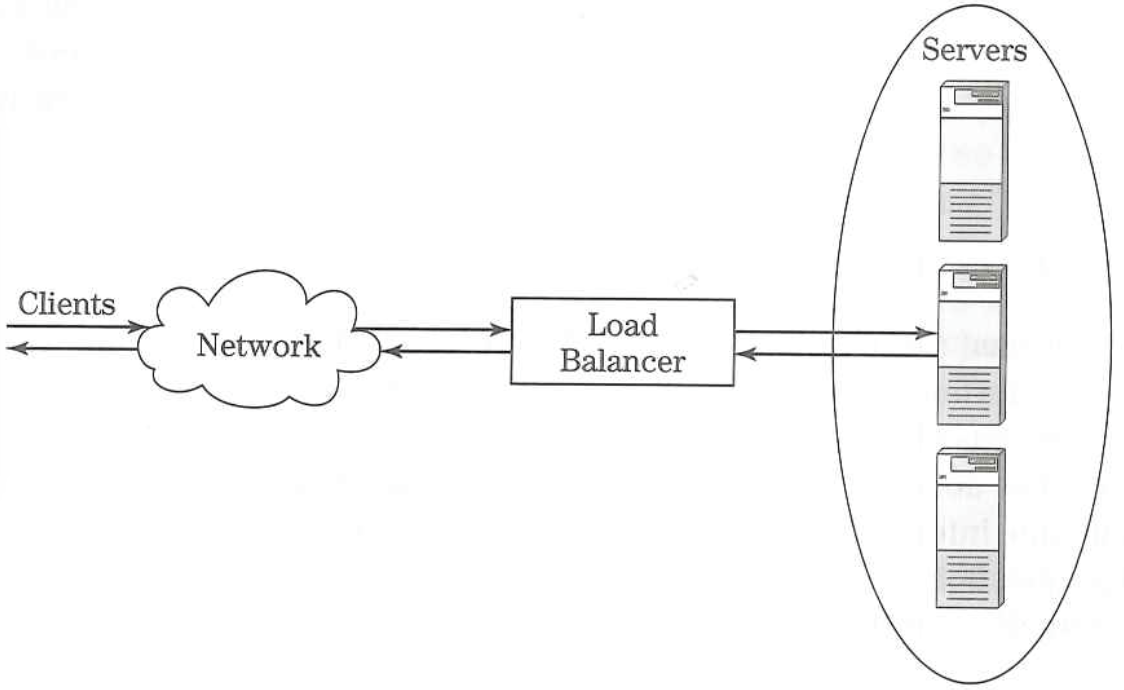
\includegraphics[width=\textwidth]{basic}\cite{lb_SFC} \\\\
	The grafic shows that the Load Balancer is the connection between the clients and the servers. The Load Blancer understands many higher-layer protocols, so they can communicate with servers intelligently. They also understand networking protocols, so they can work with the network effectively.\\\\
	Load Balancer have four big applications
	\begin{enumerate}
		\item Server load balancing
		\item Global load balancing
		\item Firewall load balancing
		\item Transparent cache switching
	\end{enumerate} 
	Server load balancing deals with multiple servers to scale beyond the capacity of one server and to handle a server failure. Global load balancing directs users to different data centers consisting of server farms so they can provide quicker response and handle a data center failure. The Firewall Load balancing can distribute load between multiple firewalls to again, handle a failure of one of them. Transparent cache switching directs traffic to caches to minimize the response time. \\ \\
	There are three main forms of products for load balancing. 
	\begin{enumerate}
		\item Software load-balancing
		\item Appliances
		\item Switches
	\end{enumerate}
	\textbf{Software load balancing} are products that run on load balancing servers. They have algorithms to coordinate the traffic among them. For example Apache Module mod\_proxy is a popular tool. Nginx would be another tool that allows software load balancing. They are mostly for free which is great if one runs on a low budget.  \\\\ % TODO: kann man noch weiter ausfuehren
	\textbf{Appliances} are a all-in-one product that include necessary hardware and software to do web switching. It may has some special operating system and custom hardware. For example Cisco has hardware appliances that handle load balancing for you. \\\\ % TODO: More examples ...	
	\textbf{Switches} have to their traditional functionality in OSI Layer 2/3, are also able to do load balancing on Layer 4-7. Mostly though, they a significant amount of work done by software. For example Zen Load Balancer  and Cisco as well have switches  appliances that handle load balancing for you.
	
	\subsection{Use Cases and Examples}
	%This section should pick up the significant points from the "Needs and Goals" and bring them in a relation with specific, real examples. S61
	
	\newpage
	\section{Basic Concepts}
	\subsection{Networking Fundamentals}
	The OSI model contains seven layers and every single one provides it's own functionality and data.\\
	If we take a closer look on the deeper layers like data link and network, which is representative for layer two and three, we can see that their header information contains IP and MAC addresses. These addresses can be used to decide where a package has to be send when it's revived by a switch.\\
	This basic concept of routing packages builds the fundament for load balancing. It's about making a decision if, and where the data has to go. \cite{lb_SFC}
	
	\subsection{Higher Layered Distribution}
	\textbf{Layer-7 Switching}\\
	Layer-7 switching, which is also known as application-level load balancing, describes a way of load distribution based on the content of the client request. Parsing the requests causes a high overhead on the balancer's side, so it's scalability is limited.\\
	The appliances which are responsible to perform layer 7 load balancing are called Application Delivery Controllers (\gls{ADC}). \gls{ADC}'s presents a "virtual sever" to the world wide web (\gls{WWW}),accepts requests and distributes them to the right application server, determined over the use of application data.\\
	\\
	The knowledge about the requested data allows to serve specific types of content. A useful distribution of content are server- and client-side-scipts for example. \cite{AppLayerBalancing}
	
	\subsection{Load-Distribution Methods}
	Summary of common load distribution Methods, their benefits and disadvantages.
	
	\newpage
	\section{Advanced Concepts}
	\subsection{Session Persistence}
	A way of load distribution where the balancer has to store the whole session information during the time of an application transaction is called Session Persistence. In addition to the right client address the balancer also has to know about the correct server, the request got forwarded to. This concept is mostly used on web services where the server has to respond with user specific content or data.\\
	For Example you can imagine an on-line book store which provides a shopping cart function that keeps your articles during your stay. If the load balancer would not store the session information during your purchase the selected article would probably get lost or in the worst case inverted with the goods of another user.\\
	The way to get the information which is needed is broadly based onto two sources:\\
	\\
	\textbf{TCP SYN Packet}\\
	TCP SYN is the first request the clients sends to the server if he wants to establish a new connection.\\
	It contains the source IP address and port to identify the user and also the destination Ip and port to identify the server.\\
	\\
	\textbf{Application Request}\\
	If the user calls an application or a method on the server the request has to be defined in the send packages.\\
	This information is used by the balancer to forward the request to the right providing server.
	
	\subsection{URL Switching}
	%The flexibility of layer seven load balancing and the included url switching.
	Services which provide a huge amount of information may have the problem that a single server cant hold the whole available content. The content has to be divided among a few servers and therefore URL Switching is used.\\
	Servers which are responsible for the same kind of information can be combined to a group. This makes it more easy to address the distributed contents and map the appropriate requests.
	The requested content from the client gets identified by names or values in the URL. This is accomplished by specifying the URL switching policies on the load balancer.\\
	\\
	\textbf{Seperating Static and Dynamic Content}\\
	Another way of URL switching is to separate the static and dynamic content in server farms. Static content is defined as information that does not change very often and can be separated from the dynamic content which may has to be generated per request.\\
	\\
	\textbf{Current URL and Cookie Switching}\\
	After our balancer has detected what server group to choose because of the requested URL we might need a way to stay in communication with the content server. Therefore a cookie-read method can be used whereby a cookie gets inserted from the server which can be read from the balancer.
	If no cookie is found the load balancer detects the request as new session and returns to it's URL switching policy.
	
	\subsection{Network-Address Translation}
	Fast Layer 4 load balancing and the appliance as default gateway.
	
	\newpage
	\section{Scheduling Algorithms}
	\subsection{Round-Robin}
	This is one of the simplest scheduling algorithms. The load distribution happens on every server equally. If this method is used all the servers should have the same capacity. If this is not the case it can mean that a less powerful server receives the next request even though it isn't able to manage it. This could case a overload on the weaker servers in the system. 
	
	\subsection{Weighed Robin-Round}
	This scheduling algorithms is based on Robin Round. Additionally it has a weight distribution on each server. The administer gives the servers a certain weight and including this, the request are spread. This method takes in account that the servers may have different performance. 
		
	\subsection{Last Connection}
	The last two algorithms didn't include the length of the connections. If a weak server only gets a certain amount of weight but those requests stay longer, it still can have an overload. To avoid this problem this method gives the requests to the server with the least connections. "The server  in the cluster with the least number of active connections automatically receives the next  request. Basically, the same principle applies here as for the simple round robin: The servers  related to a Virtual Service should ideally have the similar resource capacities."\cite{schedu} However, in low traffic rates, it is now balanced out because the first server will be preferred. This happens due to the equality of the servers. The first sever will always be selected as long as he has continually active traffic. 
	
	\subsection{Least Connected Slow- Start Time}
	This algorithm provides a "ramp-up time" for new servers in the system. When a new sever is added, a time can be configured in which it slowly gets increasingly more requests. This way the server doesn't get overloaded by a flood of connections upon startup. The downside of this method is that it takes a while until the full potential of a new server can be used. This can be a problem if you need to add power quickly. 
	
	\subsection{Weighed Least Connection}
	This method is a combination of Last Connection and Weighted Robin Round algorithms. The Number of connection and the weight which the administer gave the servers are taking in account. The next request goes to the server with the smallest ratio between weight and connections. "The number of active connections combined with the various weights defined by the  administrator generally provides a very balanced utilization of the servers, as it employs the  advantages of both worlds. "\cite{schedu}
	
	\subsection{Agent Based Adaptive Balancing}
	Other then the methods above this contains an adaptive logic. It checks at regular intervals the servers for their traffic load. The Load Balancer periodically gets a file from the server in which their work load is stated. This works with HTTP GET function. "Each server machine should  provide a file that contains a numeric value in the range between 0 and 99 representing the  actual load on this server (0 = idle, 99 = overload,101 = failed,102 = administratively disabled)."\cite{schedu} With this information  including the weight each server has the Load Balancer can handle the traffic between the severs very sufficient. Although during a period of very low traffic the Load Balancer switches to Weighted Robin Round. This is because otherwise it would result in uncontrolled distribution.
	
	\subsection{Multiple Queue Scheduling}
	This method separates the queue into two different queues. This way the request is divided and can be worked on at the same time and later being put back together. For example a queue is cut into foreground and background task. Each of these queue can have their own scheduling algorithms. So the first one can use the Robin Round and second one First Come First Server. However, the two queues also have to be scheduled and put back together. 
	
	
	%\subsection{Weighted Balance}
	%Ways to guarantee a weighted balance in busy systems.
	%\subsection{Priority}
	%The meaning of priorities concerning the process of load balancing and how to route traffic to a preferred link, as long it's available.
	%\subsection{Overflow}
	%How to prevent traffic flow from slowing down when the connection runs out of available bandwidth.
	%\subsection{Persistance}
	%Eliminate session termination issue for HTTPS, E-banking, and other secure websites.
	%\subsection{Round-Robin}
	%A closer explanation to the scheduling procedure "Round Robin"
	
	\newpage
	\section{Caches}
	\subsection{Definition}
	Define what a cache is for when we talk about load balancing.
	\subsection{Types}
	The different types of caches and their usage as well as benefits and disadvantages.
	\subsection{Deployment}
	Examples and explanation how to deploy load distribution using caches.
	
	\newpage
	\section{Problems}
	\subsection{Mega Proxy Session}
	The mega proxy session which is also known as mega proxy problem describes the issue of not being able to determine the correct source IP of an user. This can be caused when the client is located behind a proxy server which determines the client connection, changes the source IP to it's own address and opens a new connection to the actual destination IP.\\
	Most ISPs and enterprises deploy proxy servers in their network to protect their client's identities but this can raise a session-persistence and therefore a load balancing problem on the balancer's side.\\
	
	\todo{Scan the image again!!}
	\begin{figure}[h!]
		\centering
		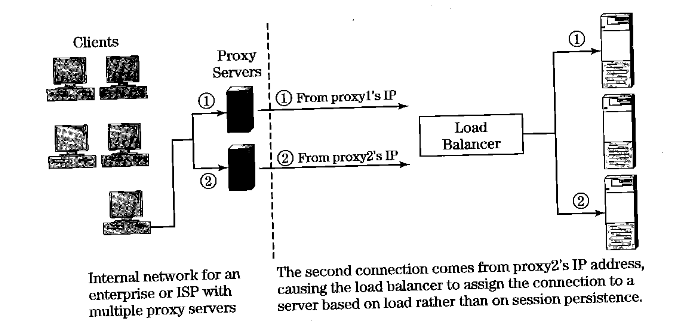
\includegraphics[width=0.7\textwidth]{img/SessionPersistanceProblem.png}
		\caption{Session persistence problem with megaproxy}
		%\label{fig:MegaProxyProblem}
	\end{figure}
	
	To avoid this problem the balancer can not longer rely on the source IP address to identify the user and has to adapt it's balancing concept.\\
	The virtual sources of the proxies can be grouped to treat them as one. With this method the balancer is still able to maintain session persistence by directing all requests to a single real server. If this method is reasonable has to be decided considering the traffic scale in your network. On one hand it solves the problem of session persistence but on the other hand it can mess up your load distribution concept because all requests from the proxy network get forwarded to the same server.
	
	\newpage
	\newglossaryentry{ADC} {
		name= ADC,
		description= {Application Delivery Controller}
	}
	\newglossaryentry{WWW} {
		name= WWW,
		description= {World Wide Web}
	}
	\printglossaries
	
	\newpage
	\bibliographystyle{plain}
	\bibliography{Loadbalancing_Haidn_Schrack.bib}
	
	\newpage
	\section{Sources}
	\todo{Please note that this is just an overview about our collected references so far, to find them in the TU-Library. We'll add our last visits during this elaberation.}
	Titel:    Load balancing servers, firewalls, and caches : [timely, practical, reliable]\\
	Autor:    Chandra Kopparapu\\
	Jahr:    2002\\
	ISBN:    ISBN 0-471-41550-2\\
	TUWS:    DAT:964, DAT:224\\
	\\
	Titel:    Dynamic load balancing : an overview\\
	Autor:    Arnold R. Krommer ; Christoph W. Ueberhuber\\
	Jahr:    1992\\
	ISBN:     -\\
	TUWS:    DAT:351\\
	\\
	Titel:    Dynamischer Lastausgleich in Parallelrechnersystemen : genetische Algorithmen und eine spezielle Rechnerstruktur\\
	Autor:    Michael Witt\\
	Jahr:    1997\\
	ISBN:    -\\
	TUWS:    -\\
	\\
	Titel:    Optimal load balancing in distributed computer systems\\
	Autor:    Hisao Kameda\\
	Jahr:    1997\\
	ISBN:    ISBN 3-540-76130-6\\
	TUWS:     -\\
	\\
	\\
	Titel:     Server Load Balancing\\
	Autor:     Tony Bourke\\
	Jahr:     August 2001\\
	0-596-00050-2, Order Number: 0502\\
	200 pages, 34.95 USD\\
	Link: http://oreilly.com/catalog/serverload/chapter/ch07.html\\
	\\
	\\
	Onlinequellen:\\
	\\
	Name:    Optimal Load Balancing in Distributed Computer Systems\\
	Link:    http://bookzz.org/book/2092081/f777c1\\
	\\
	Name:    Spectral Methods for Efficient Load Balancing Strategies\\
	Link:    http://cs.emis.de/LNI/Dissertation/Dissertation3/GI-Dissertations.03-3.pdf\\
	\\
	Name:    Lastverteilung auf dem Konzept des virtuellen Servers\\
	Link:    http://www.nm.ifi.lmu.de/pub/Fopras/fikr02/PDF-Version/fikr02.pdf\\
	\\
	Name: Dynamic Load Balancing and Scheduling\\
	Link: http://www2.cs.uni-paderborn.de/cs/ag-monien/RESEARCH/LOADBAL/\\
	\\
	
\end{document}